\documentclass[
  captions=tableheading,
  bibliography=totoc, 
  titepage=firstiscover,
]{scrartcl}

\usepackage{blindtext} %neuer input

\usepackage{longtable} % Tabellen über mehrere Seiten

\usepackage[utf8]{inputenc} %neuer input

\usepackage{scrhack}

\usepackage[aux]{rerunfilecheck} %Warnung falls nochmal kompiliert werden muss

\usepackage{fontspec} %Fonteinstellungen

\recalctypearea{}

\usepackage[main=ngerman]{babel} %deutsche Spracheinstellung

\usepackage{ragged2e} %neuer input

\usepackage{amsmath, nccmath}

\usepackage{amssymb} %viele mathe Symbole

\usepackage{mathtools} %Erweiterungen für amsmath


\DeclarePairedDelimiter{\abs}{\lvert}{\rvert}
\DeclarePairedDelimiter{\norm}{\lVert}{\rVert}

\DeclarePairedDelimiter{\bra}{\langle}{\rvert}
\DeclarePairedDelimiter{\ket}{\lvert}{\rangle}

\DeclarePairedDelimiterX{\braket}[2]{\langle}{\rangle}{
#1 \delimsize| #2
}

\NewDocumentCommand \dif {m}
{
\mathinner{\symup{d} #1}
}


\usepackage[
  math-style=ISO,
  bold-style=ISO,
  sans-style=italic,
  nabla=upright,
  partial=upright,
  warnings-off={
    mathtools-colon,
    mathtools-overbracket,
  },
]{unicode-math}

\setmathfont{Latin Modern Math}
\setmathfont{XITS Math}[range={scr, bfscr}]
\setmathfont{XITS Math}[range={cal, bfcal}, StylisticSet=1]


\usepackage[
  locale=DE,
  separate-uncertainty=true,
  per-mode=reciprocal,
  output-decimal-marker={,},
]{siunitx}

\usepackage[autostyle]{csquotes} %richtige Anführungszeichen

\usepackage{xfrac}

\usepackage{float}

\floatplacement{figure}{htbp}

\floatplacement{table}{htbp}

\usepackage[ %floats innerhalb einer section halten
  section,   %floats innerhalb er section halten
  below,     %unterhalb der Section aber auf der selben Seite ist ok
]{placeins}

\usepackage[
  labelfont=bf,
  font=small,
  width=0.9\textwidth,
]{caption}

\usepackage{subcaption} %subfigure, subtable, subref

\usepackage{graphicx}

\usepackage{grffile}

\usepackage{booktabs}

\usepackage{microtype} %Verbesserungen am Schriftbild

\usepackage[
backend=biber,
]{biblatex}

\addbibresource{../lit.bib}

\usepackage[ %Hyperlinks im Dokument
  german,
  unicode,
  pdfusetitle,
  pdfcreator={},
  pdfproducer={},
]{hyperref}

\usepackage{bookmark}

\usepackage[shortcuts]{extdash}

%\usepackage{warpcol}


\begin{document}
    \title{ATP Übungsblatt 5}
    \author{  
    Tobias Rücker\\
    \texorpdfstring{\href{mailto:tobias.ruecker@tu-dortmund.de}{tobias.ruecker@tu-dortmund.de}
    \and}{,} 
    Paul Störbrock\\
    \texorpdfstring{\href{mailto:paul.stoerbrock@tu-dortmund.de}{paul.stoerbrock@tu-dortmund.de}}{}
    }
\maketitle
\center{\Large Abgabegruppe: \textbf{Mittw. 10-12 Uhr}}
\thispagestyle{empty}

\newpage
\tableofcontents
\thispagestyle{empty}
\newpage

\setcounter{page}{1}

\section{Aufgabe 13}

    \begin{figure}[H]
        \centering
        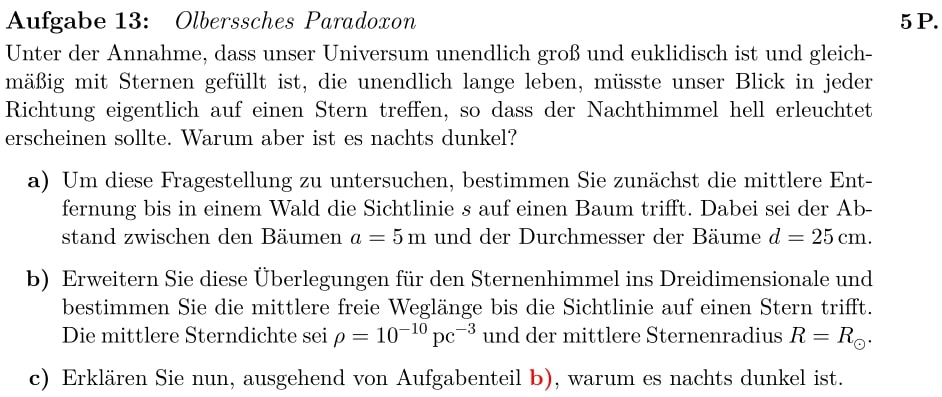
\includegraphics[width=\textwidth]{images/Aufgabe13.jpg}
        \label{fig:1}
    \end{figure}

\subsection{a)}

\subsection{b)}

\subsection{c)}

\section{Aufgabe 14}

    \begin{figure}[H]
        \centering
        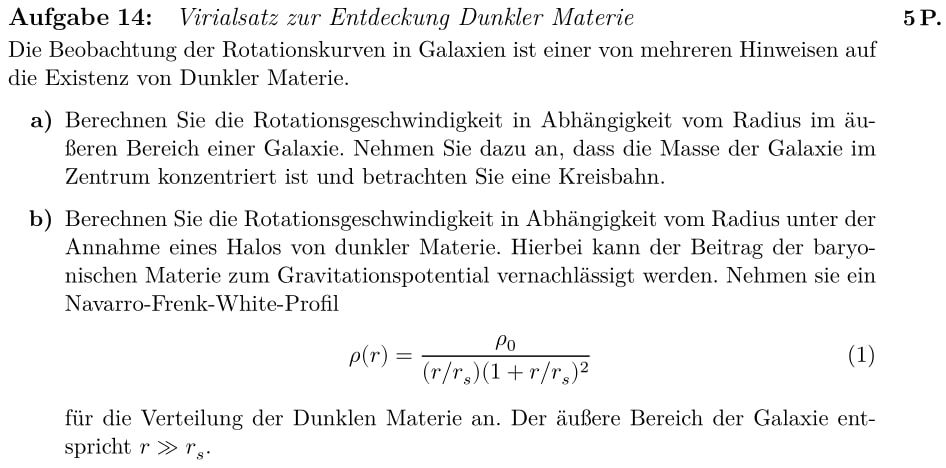
\includegraphics[width=\textwidth]{images/Aufgabe14ab.jpg}
        \label{fig:2}
    \end{figure}

    \begin{figure}[H]
        \centering
        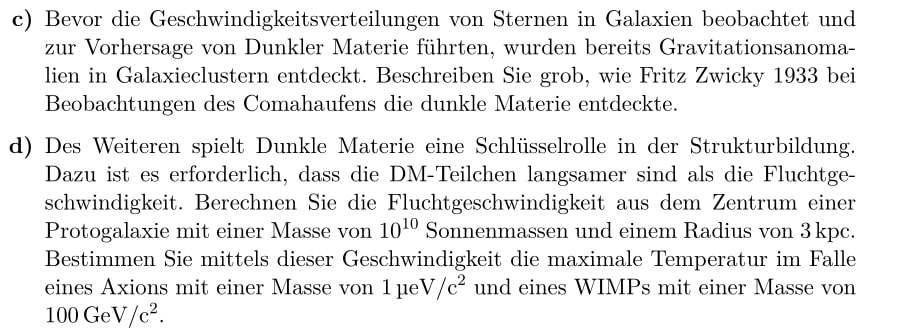
\includegraphics[width=\textwidth]{images/Aufgabe14cd.jpg}
        \label{fig:3}
    \end{figure}

\subsection{a)}
\begin{align}
    m \frac{v^2}{r} &= \frac{GMm}{r^2}\\
    v &= \sqrt{\frac{GM}{r}}
\end{align}

\subsection{b)}
\begin{align}
    M &= \int_0^{2 \pi} \int_0^{\pi} \int_0^r r^{2'} \sin \theta \rho(r') \,\dif{r'} \\
    &= 4 \pi \int_0^r r^{'2} \frac{\rho_0}{(\frac{r'}{r_s})(1+\frac{r'}{r_S})} \dif{r'} \\
    &= 4 \pi \rho _0 r_s \int_0^r \frac{r'}{(1+\frac{r'}{r_s)}^2} \,\dif{r'} \\
    &= 4 \pi \rho _0 r_s^3 \int_^r \frac{r'}{(r_s+r')^2} \,\dif{r'}\\
    \intertext{
        Substitution:
    }
    r_s+r'&=u\\
    \frac{\dif{u}{\dif{r'}}} &= 1\\
    \intertext{
        weiter
    }
    &= 4 \pi \rho _0 r_s^3 \int_{r_s}^{r_s +r} \frac{u-r_s}{u^2} \dif{u}\\
    &= 4 \pi \rho _0 r_s^3 \int_{r_s}^{r_s+r} \frac{1}{u} - \frac{r_s}{u^2} \dif{u} \\
    &= 4 \pi \rho _0 r_s^3 (\ln(u)+ \frac{r-s}{u} )\vert _{r_s}^{r_s+r}\\
    4 \pi \rho _0 r_s^3 (\ln(\frac{r_s+r}{r_s})-\frac{r}{r+r_s})
    \intertext{
        Für M in Aufgabenteil a einsetzen
    }
    \Rightarrow v &= \sqrt{\frac{G 4 \pi r_s^3 (\ln(\frac{r_s+r}{r_s}-\frac{r}{r+r_s})){r}}}
\end{align}


\subsection{c)}
\flushleft{Fritz\,}\justifying Zwicky hatte die Relativbewegungen von Galaxien im Coma-Haufen betrachtet,
da viel Masse schnelle Bewegung der Galaixien hervorruft. Über die Bestimmung
der Geschwindigkeitsdispersion und das Virialtheorem lässt sich dann die Masse des Coma-Haufens zu berechnen.
Das Masse-Leuchtkraft-Verhältnis für den Coma-Haufen ergab sich zu $250 M_{\odot}/L_{\odot} $. Für typische Sterne
in Galaxien gilt ein Verhältnis von $2,5 M_{\odot}/L_{\odot} $

\subsection{d)}


\section{Aufgabe 15}

    \begin{figure}[H]
        \centering
        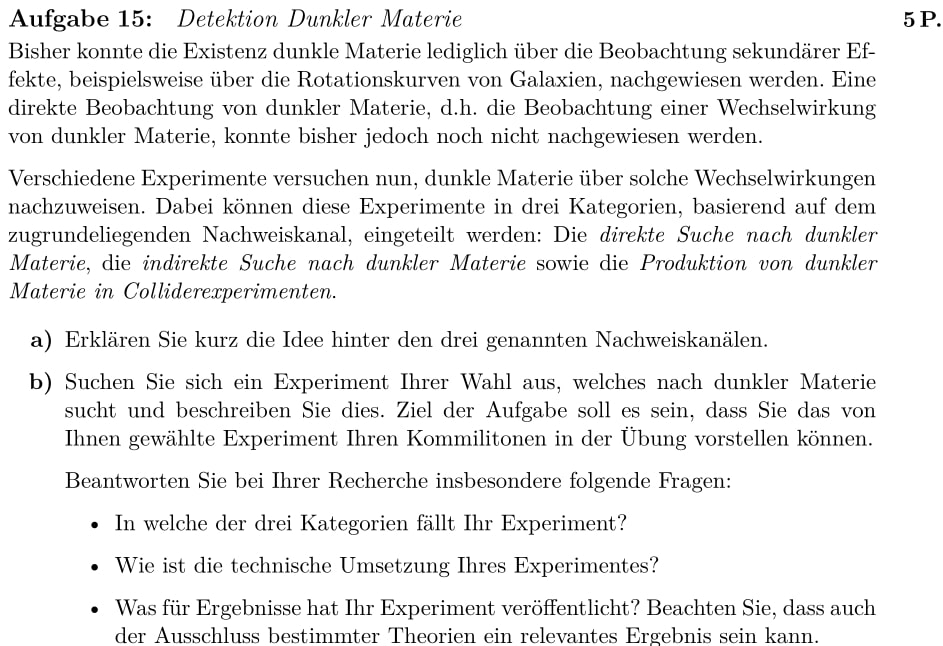
\includegraphics[width=\textwidth]{images/Aufgabe15.jpg}
        \label{fig:4}
    \end{figure}

\subsection{a)}

\subsection{b)}

\end{document}